%\documentclass[10pt]{amsart}
\documentclass[12pt]{amsart}
\usepackage[centertags]{amsmath}
\usepackage{amsfonts,amssymb}
\usepackage{enumerate}
\usepackage[sort&compress,numbers]{natbib}
\usepackage{hyperref}
\usepackage{doi}
\usepackage[latin1]{inputenc}

\usepackage{amsfonts,amsmath,amssymb,graphicx,color,amsthm}
\usepackage{tgtermes}

\textheight 8.5in
\textwidth 15cm
\oddsidemargin 0.75cm

\DeclareMathOperator{\sgn}{sgn}

\def\EE{\mathbb{E}}\def\PP{\mathbb{P}}

\begin{document}

\title{Noise-induced transitions between meta-stable atmospheric jets}
\date{\today}
\author{Tobias Grafke}

\begin{abstract}
  We analyze the occurrence of jets in the quasi-linear approximation
  of the quasi-geostrophic equations in the $\beta$-plane. The
  occurrence of a time-scale separation between zonal jets and
  non-zonal turbulent fluctuations gives raise to a law of large
  numbers, which allows us to compute the meta-stable jet solutions
  numerically. Similarly, large time-scale separations give raise to a
  large deviation principle, which in principle gives insight into
  noise-induced transitions between the fixed points. We use this fact
  to numerically compute the transition state, i.e. the point at which
  the noisy dynamics are most likely to cross the separatrix between
  the respective basins of stability of the deterministic dynamics.
\end{abstract}

\maketitle

\section{The quasi-geostrophic equation in the $\beta$-plane}

We consider 2D stochastically forced barotropic $\beta$-plane
turbulence,
\begin{equation}
  \label{eq:qg}
  \partial_t \omega + \vec{v}\cdot \nabla \omega + \beta v =
  -\lambda\omega - \nu (-\Delta)^p \omega + \sqrt{\gamma}\eta\,,
\end{equation}
in a periodic domain, $(x,y)\in[0,L]^2$, and where $\vec{v}=(u, v) =
e_z \times \nabla \psi$ is the velocity field for a stream function
$\psi(x,y)$, $\omega = \Delta \psi$ is the vorticity. Physically,
Ekman damping is present with a coefficient $\lambda$, while $\beta$
denotes the local latitude of the planetary surface. Evolving
turbulence in this setup transfers energy into zonal shear modes
\cite{rhines:1975} depending on the value of $\beta$, which is the
basis of understanding zonal jets in planetary atmospheric
dynamics. The forcing $\eta$ is supposed to act only on concentrated
modes around the forcing wave number $k_*$ as is common in 2D
turbulence \cite{lilly:1969}, but less physically motivated in the
atmosphere dynamics case \cite{srinivasan-young:2011}. In particular,
we consider $\EE\left[\eta(\vec r_1, t_1)\eta(\vec
  r_2,t_2)\right]=\delta(t_2-t_1) \chi(|\vec r_2- \vec r_1|)$.

\subsection{Rescaling into non-dimensional coordinates}
\label{ssec:rescale}

Following \cite{bouchet-nardini-tangarife:2013}, we want to
non\-dimen\-sionalize the parameters. We assume the temporal white noise
$\eta$ to be normalized such that $-2\pi^2 L^2 (\Delta^{-1}\chi)(0)=1$
(since $\eta$ forces vorticity, but energy is measured based on
velocity). Consequently, the energy input rate is $\gamma$. Neglecting
(hyper-)viscosity, the stationary energy balance yields
$E\approx\frac{\gamma}{2\lambda}$.

We now want to rescale to non-dimensional parameters such that the
average energy is unity and the domain size is $[0,2\pi]^2$. Define
the non-dimensional time $\tau=L^2\sqrt{2\lambda/\gamma}$ and
$x'=x/L$, $t'=t/\tau$. Rescale $\omega'=\tau\omega$, $v'=\tau v/L$,
$u'=\tau u$, $\beta' = L\tau\beta$ and $\nu' = \nu\tau L^{-2p}$. The
forcing correlation has to be rescaled $\chi'(r')=L^4 \chi(r)$, and define
$\alpha=\tau\lambda$. Inserting all this into equation~\eqref{eq:qg},
we arrive at
\begin{equation}
  \label{eq:qg_rescaled}
  \partial_t \omega + \vec{v}\cdot \nabla \omega + \beta v =
  -\alpha\omega - \nu (-\Delta)^p \omega + \sqrt{2\alpha}\eta\,,
\end{equation}
where all primes have been dropped. The forcing pre-factor comes from
rescaling time and the spatial forcing correlation as follows:
$\sqrt{\gamma}\tau^2 (\tau^{-1/2}L^{-2}) = \sqrt{2\alpha}$. We now
have reduced the system~\eqref{eq:qg} down to two dimensionless
parameters $\alpha, \beta$.

\subsection{Quasi-linear approximation}

A point was made in \cite{bouchet-nardini-tangarife:2013}, that the
parameter $\alpha$ actually describes a time-scale separation between
the slow zonal modes and the fast non-zonal fluctuations. Accordingly,
we split vorticity and velocity in equation~\eqref{eq:qg_rescaled}
into zonal and non-zonal components, while assuming a time-scale
separation of $\sqrt{\alpha}$ between the zonal mean quantities and
the fast fluctuations. More concretely, we set
\begin{equation}
  \label{eq:split}
  \omega = \Omega + \sqrt{\alpha}\tilde\omega,\qquad u = U + \sqrt{\alpha}\tilde u,\qquad v = \sqrt{\alpha}\tilde v\,,
\end{equation}
where $\Omega(y)=\frac1L\int \omega(x,y)\,dx$, $U(y)=\frac1L\int
u(x,y)\,dx$ and $\int v(x,y)\,dx=0$ because of periodicity. We will
drop the tilde in the following and write $\overline{ f}$ for
averaging over the $x$-coordinate, $\int f(x,y)
dx/L$. Inserting~\eqref{eq:split} into equation~\eqref{eq:qg_rescaled}
and subsequently averaging over $x$, we obtain
\begin{equation*}
  \partial_t \Omega = -\alpha \overline{v\omega} - \alpha\Omega -\nu(-\partial_y^2)^p\Omega\,.
\end{equation*}
Subtracting this equation from the full one, we obtain an equation for
the non-zonal components,
\begin{equation*}
  \partial_t \omega = -U\partial_x\omega - v\partial_y\Omega-\sqrt{\alpha}\nabla\cdot(\vec v \omega)-\alpha\omega-\beta v\,.
\end{equation*}

In the following, we neglect the non-linear interaction term of the
non-zonal component. Since $\Omega(y)=-\partial_yU(y)$, we arrive at
the quasi-linear approximation
\begin{equation}
  \label{eq:ql}
  \begin{cases}
    \partial_t U = \alpha \overline{v\omega}-\alpha U -\nu(-\partial_y^2)^p U\\
    \partial_t \omega = -U\partial_x \omega-(\partial_y^2 U-\beta)v-\alpha\omega-\nu(-\Delta)^p\omega+\sqrt{2}\eta\,.
  \end{cases}
\end{equation}
The kinetic theory of this equation is treated in
\cite{bouchet-nardini-tangarife:2013}. Computing the correlation
$\EE\left[\omega(y_1)\omega(y_2)\right]$ (equivalently, second
cumulant) instead of $\omega$ in equation~\eqref{eq:ql}, we recover
CE2 \cite{marston-conover-schneider:2008} or equivalently S3T by
\cite{farrell-ioannou:2003, farrell-ioannou:2007}. This also opens the
possibility to analyze emergence and stability of the jets in some
detail via linear stability analysis in the context of atmosphere
dynamics \cite{bakas-ioannou:2011, bakas-ioannou:2013} and in the
context of plasma physics \cite{parker-krommes:2013,
  parker-krommes:2014}.

\section{Meta-stable atmospheric jet solutions and large time-scale separation}

It is possible to find parameter ranges in which the quasi-linear
approximation (and, hopefully, the fully non-linear
system~\eqref{eq:qg}) has multiple stable fixed points of the
deterministic dynamics, corresponding to meta-stable jet solutions. In
the following, we want to analyze how we compute these fixed points
numerically in an efficient way. Furthermore, the limit of large
time-scale separation gives raise to a large deviation principle,
which allows us to characterize the transition and numerically compute
transition states.

\subsection{Large time-scale separation}

The system of equations~\eqref{eq:ql} shows how $\alpha$ can be interpreted as
time-scale separation. If we rescale the time by $\alpha$ (and replace
the unimportant viscosity $\nu$ with $\alpha\nu$, and
$\sigma\sigma^\dagger=\chi$), we obtain
\begin{equation}
  \begin{cases}
    \partial_t U = \overline{v\omega}- U -\nu(-\partial_y^2)^p U\\
    d \omega = -\frac{1}{\alpha}\Gamma(U)\omega\,dt  + \sqrt{\frac{2}{\alpha}} \sigma dW
  \end{cases}
\end{equation}
where the second line is a stochastic PDE and an Ornstein Uhlenbeck
process with drift 
\begin{equation}
  \Gamma(U) = U\partial_x +(\partial_y^2 U-\beta)\partial_x \Delta^{-1} + \alpha + \nu(-\Delta)^p\,.
\end{equation}
Note that this system, under a suitable discretization, is of the form
\begin{equation*}
  \begin{aligned}
    \dot X_i &= \sum_{j,k} y_j M_{i,j,k} y_k + R X_i\\
    dy_j &= -\sum_k \Gamma_{j,k} y_k\,dt + \sum_k \sigma_{j,k} dW_k
  \end{aligned}
\end{equation*}
which has the specific form discussed in
\cite{bouchet-grafke-tangarife-etal:2016}. In particular, we will make
use of the fact that we can write down both a law of large numbers
(LLN) and a large deviation principle (LDP) in the limit $\alpha\to0$.

\subsection{Meta-stable jet configurations}

We want to analyze the meta-stable jet configurations in the limit of
large time-scale separation, $\alpha\to0$. Define the ``virtual fast
process'' $\tilde\omega_u$ by
\begin{equation}
  \label{eq:virtfast}
  d\tilde\omega_u = -\Gamma(u)\tilde\omega_u + \sqrt{2}\sigma dW\,,
\end{equation}
i.e. the non-zonal vorticity fluctuations in their natural (fast)
time-scale for a fixed zonal velocity $U=u$. Then one can show the
existence of an LLN for the mean $\bar U$, i.e. ${\PP(|U(t)-\bar
  U(t)|<\epsilon)\to1} \forall \,t,\epsilon>0$ as $\alpha\to0$. The
evolution equation for $\bar U(t)$ is given by
\begin{equation}
  \label{eq:lln}
  \begin{aligned}
    \partial_t \bar U &= \EE_{\bar U}\left[\overline{\tilde\omega_{\bar U} \tilde v_{\bar U}}\right] -\bar U - \nu (-\Delta)^p \bar U\\
    &= \frac1L\int \left(\partial_x \Delta^{-1} \EE_{\bar U}\left[\tilde\omega_{\bar U}(x,y)\tilde\omega_{\bar U}(x',y')\right]\right)_{y=y',x=x'} \,dx -\bar U - \nu (-\Delta)^p \bar U\,,
  \end{aligned}
\end{equation}
where of course $\tilde v_u$ is the velocity corresponding to the
virtual fast process. Note that assuming ergodicity we have
\begin{equation*}
  \EE_{\bar U}\left[\overline{\tilde\omega_{\bar U} \tilde v_{\bar U}}\right] = \lim_{T\to\infty}\frac1T \int_0^T \overline{\tilde\omega_{\bar U} \tilde v_{\bar U}}\,dt\,,
\end{equation*}
which implies that the solution of S3T and CE2 in the large time-scale
separation limit converges to the LLN~\eqref{eq:lln}.

Since the virtual fast process~\eqref{eq:virtfast} is an
Ornstein-Uhlenbeck process, we can write down its invariant measure
explicitly. As a consequence, the correlation matrix of the virtual
fast process, $C_{\bar U}(x,y,x',y')=\EE_{\bar U}\left[\tilde\omega_{\bar U}(x,y)
  \tilde \omega_{\bar U}(x,y')\right]$, fulfills the stationary
Lyapunov equation
\begin{equation}
  \label{eq:lyapunov}
  \Gamma(\bar U) C_{\bar U} + C_{\bar U} \Gamma(\bar U)^\dagger = 2
  \sigma \sigma^\dagger\,.
\end{equation}

We therefore conclude that the zonal dynamics $U$ in the limit of
infinite time-scale separation $\alpha\to0$ can be modeled by the
solution $\bar U$ of the LLN,
\begin{equation}
  \partial_t \bar U = \frac1L\int \left(\partial_x \Delta^{-1} C_{\bar U}(x,y,x',y')\right)_{y=y',x=x'} \,dx - \bar U - \nu (-\Delta)^p \bar U\,,
\end{equation}
where $C_{\bar U}$ is obtained from equation~\eqref{eq:lyapunov}. 

\subsection{Numerical computation of meta-stable states}

We propose the following algorithm to compute the fixed points of the
LLN efficiently. Discretize the $y$-direction with $N_y$ grid points
in real space, and the $x$-direction with $N_x$ grid points in Fourier
space, defining 
\begin{equation*}
  \omega(x,y) = \sum_{k=-N_x/2}^{N_x/2} \hat\omega_k(y) e^{2\pi i k x/L}\,,
\end{equation*}
for the Fourier-coefficients $\hat\omega_k(y)$. Since a product in
real space is a convolution in Fourier space, and since the mean
$\frac1L\int\cdot\,dx$ is the same as evaluating the $k=0$ coefficient
of the Fourier transform, we know that
$\overline{v(x,y)\omega(x,y)}=\sum_k \omega_k(y) v_{-k}(y)$. Therefore,
\begin{equation*}
  \begin{aligned}
    \frac1L\int \left(\partial_x \Delta^{-1} C_{\bar U}(y,y')\right)_{y=y',x=x'} \,dx &= \sum_{k=-N_x/2}^{N_x/2} \left( ik(\partial_y^2-k^2)^{-1} C_k(y,y')\right)_{y=y'}\\
    &= \sum_{k=0}^{N_x/2}\left( ik(\partial_y^2-k^2)^{-1} (C_k(y,y')-C_k^*(y,y')\right)_{y=y'}\\
    &= \sum_{k=0}^{N_x/2}\left( -2k(\partial_y^2-k^2)^{-1} \Im \left[C_k(y,y')\right]\right)_{y=y'}\\
    &= \sum_{k=0}^{N_x/2}\mathrm{diag}\left[ -2k(\partial_y^2-k^2)^{-1} \Im \left[C_k(y,y')\right]\right]\,,
  \end{aligned}
\end{equation*}
where $\mathrm{diag}[A]$ refers to the main diagonal of the matrix $A$
and $\Im[z]$ is the imaginary part of $z$. The matrix $\Gamma_k(U)$
separates nicely in $k$, so we can solve the Lyapunov
equation~\eqref{eq:lyapunov} independently for each $k$, and only for
those $k$ where there are forced modes present (otherwise,
$\Gamma_k=0$). In practice, one often considers spatially
homogeneous, isotropic forcing around a frequency $k_*$, so that
$||\vec k|-k_*|<\delta k$ in Fourier space (maybe furthermore restricting not
to force the zonal average, $\hat\chi(k_x=0)=0$).  The Lyapunov equation
therefore is an equation for matrices of size $n\times n$, which is of
computational complexity $\mathcal{O}(n^3)$
\cite{bartels-stewart:1972}.

The algorithm we propose in total reads
\begin{equation}
  \label{eq:num}
  \partial_t U(y) = \sum_{k=0}^{N_x/2}\mathrm{diag}\left[ -2k(\partial_y^2-k^2)^{-1} \Im \left[C_k(y,y')\right]\right] - U(y) - \nu (-\Delta)^p U(y)\\
\end{equation}
where for each $t$ and all $k$ the matrix $C_k$ is defined by
\begin{equation}
  \Gamma_k(U) C_k + C_k \Gamma_k(U)^\dagger = 2 \sigma_k \sigma_k^\dagger\,.
\end{equation}

The idea to numerically exploit the separation between macro and micro
time scales by decoupling them explicitly is reminiscent of the
heterogeneous multiscale method (HMM) \cite{e-engquist-huang:2003,
  e-engquist-li-etal:2007}.

\subsection{Numerical results}
\label{sec:fixedpoints-numerics}

\begin{figure}[t]
  \begin{center}
    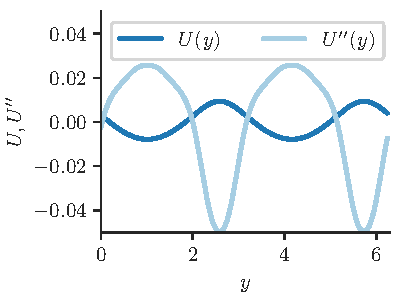
\includegraphics[height=115pt]{figures/stable-2jet}\hspace{-0.2em}
    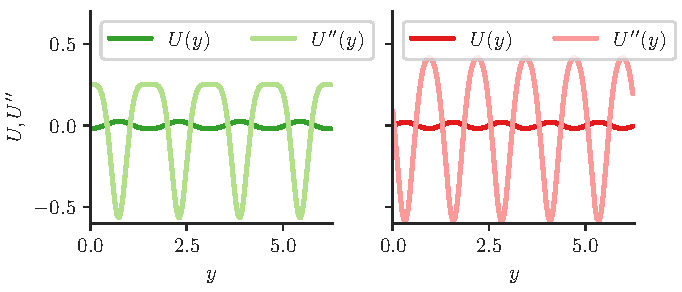
\includegraphics[height=115pt]{figures/stable-4-5-jet}
  \end{center}
  \caption{Stable configurations for different parameters of
    $\alpha,\beta$. Left: $\alpha=10^{-4}, \beta=1.6$, the 2-jet
    configuration is the only stable solution. Right:
    $\alpha=5\cdot10^{-3}, \beta=5.3$, both 4-jet (green) and 5-jet
    (red) configurations are stable.\label{fig:stable}}
\end{figure}

\begin{figure}[b]
  \begin{center}
    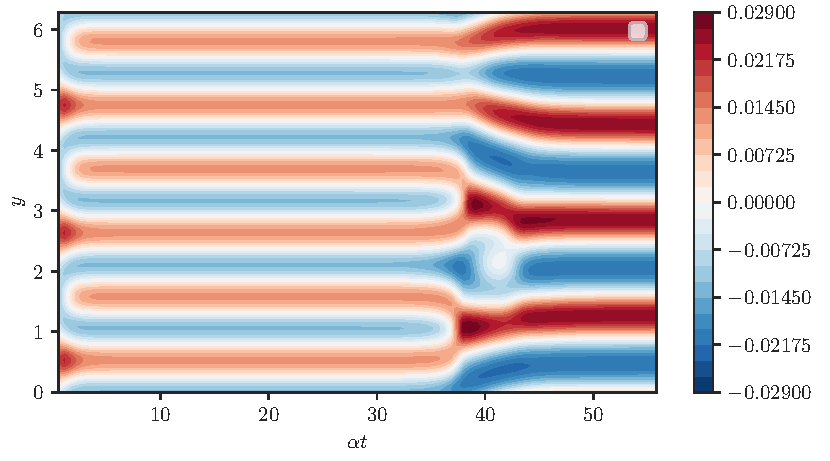
\includegraphics[width=0.9\textwidth]{figures/dynamics-4-jet}
  \end{center}
  \caption{Evolution of the LLN equation~\eqref{eq:lln}, starting at
    the (unstable) 3-jet configuration, which eventually evolves into
    the (stable) 4-jet configuration through a series of splitting and
    merging events.\label{fig:dynamics}}
\end{figure}

We can use this algorithm as a basis to find sets of parameters
$\alpha, \beta$, where the LLN allows multiple stable fixed-points by
integrating equation~\eqref{eq:num} for long times. Note that the
integration has to be done only on the slow timescale, i.e. the fast
variable does not limit the numerical stability. Note also that when
choosing an unconditionally stable integrator for the (hyper-)viscous
term, which poses the strictest stability condition on the relaxation,
we can actually view the time integration of~\eqref{eq:num} as a
pre-conditioned iterative descend algorithm to find the fixed point
$\partial_t U=0$. We use exponential time differencing for both linear
terms in~\eqref{eq:num} and obtain the fixed point of the LLN after
only a view iterations (time-steps).

In the following, use $N_x=32$, $N_y=128$, with a forcing $|\vec
k|\in[13,15]$ normalized according to section~\ref{ssec:rescale} for
different values of $\alpha, \beta$. Shown in figure~\ref{fig:stable}
are the meta-stable fixed points of the LLN in which 2 jets (left) and
both 4 or 5 jets (right) are stable. Shown in
figure~\ref{fig:dynamics} is a long-time evolution of the LLN starting
at the (unstable) 3-jet configuration, which eventually evolves into
the (stable) 4-jet configuration through a series of splitting and
merging events. Note that in this evolution, it is always the
retrograde jets that split, and always the prograde jets that merge.

\section{Noise-induced transitions between meta-stable jet configurations}

The computation of the full large deviation minimizers for the
transition trajectories is complicated. As indicated in
\cite{bouchet-grafke-tangarife-etal:2016}, there is no explicit
formula for the large deviation Hamiltonian of the complete
system. However, we can gain some insight into the merging events by
computing the heteroclinic orbit connecting different meta-stable
states. In particular, this allows a computation of the transition
state (saddle point) which must also be part of the transition
trajectory, as well as the downhill trajectory onwards from
there. This implies that we get access to the configuration at which
the separatrix between the basins of attraction of the respective
fixed points is most likely crossed in the limit $\alpha\to0$.

\subsection{Transition state and heteroclinic orbit}

The heteroclinic orbit can be computed via the string method
\cite{e-ren-vanden-eijnden:2002} by integrating the LLN equation
\eqref{eq:lln} for several images along a string connecting the
meta-stable states, while simultaneously keeping the string
artificially arc-length parametrized. More precisely, consider a
family of configurations $U_s(y)$ parametrized by $s\in[0,1]$, such
that $U_0$ and $U_1$ are two stable fixed points of the LLN
equation~\eqref{eq:lln}. Then, relax the string $U_s$ in virtual
time $\tau$ by
\begin{equation}
  \partial_\tau U_s = (1-\hat t\otimes \hat t)b(U_s)\,,
\end{equation}
where $\hat t = \partial_s U_s/|\partial_s U_s|$ is the unit tangent
vector along the string, $(1-\hat t\otimes \hat t)$ is the projector
on the component perpendicular to the string at each point, and
\begin{equation*}
    b(U_s) = \EE_{U_s}\left[\overline{\tilde\omega_{U_s} \tilde v_{U_s}}\right] -U_s - \nu (-\Delta)^p U_s  
\end{equation*}
is the dynamics of the averaged zonal velocity. When converged, this
ensures that at each point $s$ along the string we have $\partial_s
U_s \parallel b(U_s)$ and $U_s$ is the heteroclinic orbit connecting
the two stable fixed points with a saddle-point in-between. In
particular, this orbit contains the saddle point configuration $\hat U
= U_{\hat s}$, $\hat s\in(0,1)$ where the dynamics vanish, $b(\hat
U)=0$ and the only unstable direction is tangential to the
string. This saddle point also has to be contained in the minimizer
(or at least a local minimizer) of the rate function (which we don't
have access to) and corresponds to the point at which the separatrix
between the basins of stability of the LLN equation is crossed.

Note that this procedure does not allow an estimate of the relative
stability of the configurations, the transition probabilities or the
exit times. We can use the saddle-point calculation to reduce the
complexity of the full minimization somewhat, though, by only
requiring a computation of the ``uphill'' trajectory up to the saddle
point.

\subsection{Numerical computation of the transition state and heteroclinic orbit}

\begin{figure}[t]
  \begin{center}
    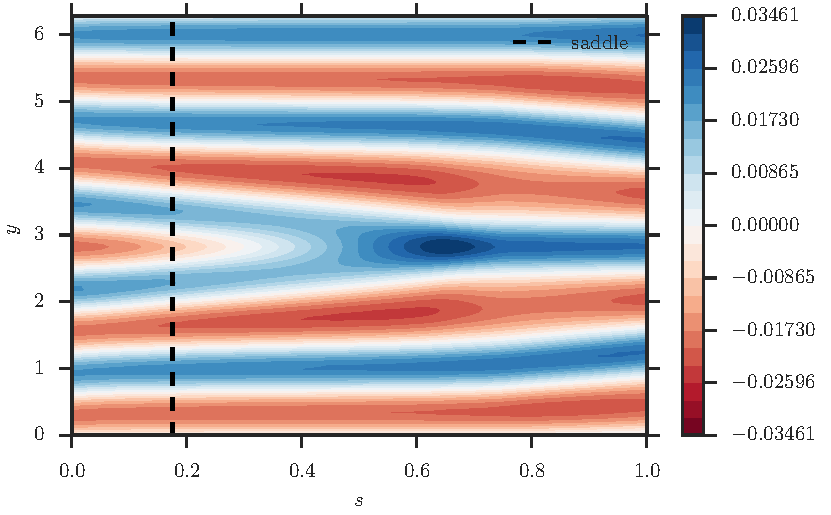
\includegraphics[width=0.9\textwidth]{figures/merger-5-to-4-string}
  \end{center}
  \caption{Heteroclinic orbit connecting the meta-stable 5-jet
    configuration $U_5$ to the meta-stable 4-jet configuration
    $U_4$. The saddle $\hat U$ is located at approximately $\hat
    s\approx0.17$.\label{fig:merger-4-to-5-string}}
\end{figure}

\begin{figure}[t]
  \begin{center}
    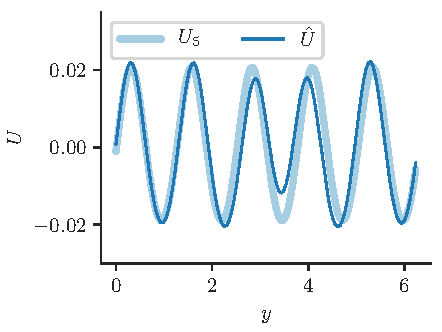
\includegraphics[width=0.6\textwidth]{figures/merger-5-to-4-saddle}
  \end{center}
  \caption{Saddle point configuration $\hat U$ in comparison to the
    5-jet configuration $U_5$.\label{fig:merger-4-to-5-saddle}}
\end{figure}

Numerically, one has to solve the Lyapunov equation
\eqref{eq:lyapunov} for each $k$ and each image along the string until
the iteration reaches a fixed point. The projection on the component
perpendicular to the string is most easily implemented by
reparametrization after every iteration.

As example case, we take the parameters $\alpha=5\cdot10^{-3},
\beta=5.3$ which exhibit locally stable 4- and 5-jet configurations as
shown in figure \ref{fig:stable} (right). The heteroclinic orbit
connecting these two configurations $U_4$ and $U_5$ is shown in figure
\ref{fig:merger-4-to-5-string}. Here, $s\in[0,1]$ denotes the string
parameter, with $U(s=0)=U_5$ and $U(s=1)=U_4$. The corresponding
saddle point configuration can be identified at roughly $\hat
s\approx0.17$, where $b(\hat U)$ close to zero. It is depicted in
figure \ref{fig:merger-4-to-5-saddle} in comparison to $U_5$.

Note that in contrast to the results of Bouchet and Simonnet
\cite{bouchet-rolland-simonnet:2019} I am only able to find a single
saddle point, namely the one where a prograde jet merges/splits, not
the one where a retrograde merges/splits. This is regardless of the
initial condition from which the string relaxes, and in particular
also applies to the case where I intentionally start with a retrograde
split initial condition. In contrast, the results obtained from
adaptive multilevel splitting (AMS)
\cite{bouchet-rolland-simonnet:2019} seem to suggest that forward- and
backward transition appear to split retrograde jets, but merge
prograde jets (which is in agreement with the deterministic behavior
of section~\ref{sec:fixedpoints-numerics}), and the transition
trajectories share no points except the equilibria. It is not clear
whether this points to a systematic difference or is simply the
consequence of different parameters. The location of the saddle points
in the AMS simulations is somewhat unclear, as well.

The numerical parameters are $N_x=32, N_y=128$ for each image, with
$N_{\text{images}}=128$ and a number of iterations of roughly
$N_{\text{iter}}\approx10^2$.

%% BIBLIOGRAPHY %%

\bibliographystyle{unsrtnat} \bibliography{bib}

\end{document}
